\section{Theorie}
\label{sec:Theorie}

Ein Lock-In-Verstärker dient zur Messung verrauschter Signale. 
Diese werden mit einem Referenzsignal moduliert, welches eine Referenzfrequenz $\omega_0$ und Phase besitzt.
Der Verstärker besteht aus einem Bandpass- und einem Tiefpassfilter und einem Phasenverschieber, wie in Abbildung (1) zu erkennen ist.

\begin{figure}[H]
  \centering
  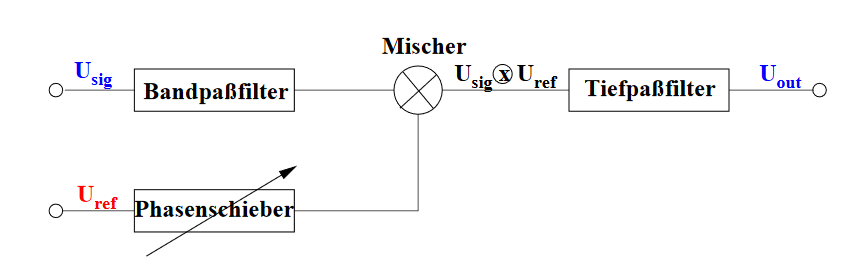
\includegraphics[height=5cm]{theorie.png}
  \caption{Wichtige Bestandteile eines Lock-In-Verstärker. \cite[S. 1]{l}}
\end{figure}

\noindent Zuerst wird das verrauschte Signal $U_\text{sig}$ von hohen und niedrigen Frequenzen durch den Bandpassfilter befreit.
Ein Mischer dient dazu, das Signal mit der Frequenz $\omega_0$ des Referenzsignals zu multiplizieren.
Mit einem Phasenverschieber kann die Phase $\phi$ des verrauschten Signals mit der Phase des Referenzsignals synchronisieren ($\Delta \phi = 0$).
Der Tiefpass ($\tau = RC \gg 1\ \omega_0 $) integriert das Mischsignal.
Die Rauschbeiträge werden sich so weit herausmitteln, dass die Ausgangsspannung proportional zur Eingangspannung ist($U_\text{out} \propto U_0 cos\phi $).
Wählt man die Zeitkonstante $\tau = RC$ sehr groß, kann man die Bandbreite $\nu = 1/(\pi RC)$ klein wählen.
Damit kann eine hohe Güte von $Q = 100000$ erreicht werden.

\noindent Als Beispiel wird in Abbildung (2) eine sinusförmige Signalspannung mit einer Rechteckspannung, welche als eine Fourierreihe mit ungeraden Oberwellen dargestellt werden kann und die gleiche Frequenz besitzt, moduliert.
Das Produkt der beiden Freqzenzen enthält nur die geraden Oberwellen der Grundfrequenz $\omega$. 
Wird der Tiefpassfilter so gewählt, dass er die Oberwellen unterdrückt, erhält man eine Gleichspannung porportional zur Signalspannung
\begin{align}
U_\text{out} = \frac{2}{\pi} U_0 .
\end{align}
Sind die Spannungen nicht in Phase, ergibt sich
\begin{align}
U_\text{out} = \frac{2}{\pi} U_0 cos \phi .
\end{align}

\begin{figure}[H]
  \centering
  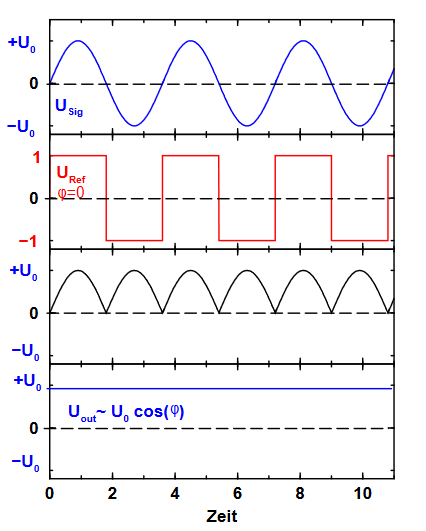
\includegraphics{bsp.png}
  \caption{Verläufe des verrauschten Signals, der Referenzspannung, des Mischsignals, und der integrierten Spannung.  \cite[S. 2]{l}}
\end{figure}
